\documentclass{article}

% If you're new to LaTeX, here's some short tutorials:
% https://www.overleaf.com/learn/latex/Learn_LaTeX_in_30_minutes
% https://en.wikibooks.org/wiki/LaTeX/Basics

% Formatting
\usepackage[utf8]{inputenc}
\usepackage[margin=1in]{geometry}
\usepackage[titletoc,title]{appendix}

% Math
% https://www.overleaf.com/learn/latex/Mathematical_expressions
% https://en.wikibooks.org/wiki/LaTeX/Mathematics
\usepackage{amsmath,amsfonts,amssymb,mathtools}

% Images
% https://www.overleaf.com/learn/latex/Inserting_Images
% https://en.wikibooks.org/wiki/LaTeX/Floats,_Figures_and_Captions
\usepackage{graphicx,float}
\usepackage{caption}
\usepackage{subcaption}

% Tables
% https://www.overleaf.com/learn/latex/Tables
% https://en.wikibooks.org/wiki/LaTeX/Tables

% Algorithms
% https://www.overleaf.com/learn/latex/algorithms
% https://en.wikibooks.org/wiki/LaTeX/Algorithms
\usepackage[ruled,vlined]{algorithm2e}
\usepackage{algorithmic}

% Code syntax highlighting
% https://www.overleaf.com/learn/latex/Code_Highlighting_with_minted
\usepackage{minted}
\usemintedstyle{borland}
\usepackage{listings}


% References
% https://www.overleaf.com/learn/latex/Bibliography_management_in_LaTeX
% https://en.wikibooks.org/wiki/LaTeX/Bibliography_Management
\usepackage{biblatex}
\addbibresource{references.bib}

% Title content
\title{AMATH 482 Homework 2}
\author{Rishabh Verma}
\date{February 10th, 2021}

\begin{document}

\maketitle

% Abstract
\begin{abstract}
    %
\end{abstract}

% Introduction and Overview
\section{Introduction and Overview}
The MNIST dataset contains labeled scans of handwritten digits. Each scan is a 28x28 pixel image, and each pixel is an 8-bit greyscale value. Each image contains a size-normalized centered digit. There are 60,000 scans in the training set and 10,000 scans in the testing set.


%  Theoretical Background
\section{Theoretical Background}
\subsection{Limitations of Discrete Fourier Transform}
The Discrete Fourier Transform is a method to decompose a signal into its constituent frequencies. It is given by the formula for all bins $k = -N/2,...,N/2-1$: 

\begin{equation}
	\hat{x}_k = \dfrac{1}{N}\sum_{n=0}^{N-1} x_n e^{\tfrac{2\pi i k n}{N}}
	\label{eqn:fourier}
\end{equation}

where $x_n$ represents a signal. The DFT is subject to aliasing, in that

\begin{equation}
	\hat{x}_k = \hat{x}_{k+\mu k} \text{ for all integers } \mu,
	\label{aliasing}
\end{equation}

and this will be used to show the following result. If a periodic signal $x_n$ is shifted in time, i.e. there exists some non-zero integer $\tau$ and a shifted signal $y_n = x_{n-\tau}$, then 

\begin{equation}
	\begin{split}
		\hat{y}_k &= \dfrac{1}{N}\sum_{n=0}^{N-1} y_n e^{\tfrac{2\pi i k n}{N}}=\dfrac{1}{N}\sum_{n=0}^{N-1} x_{n-\tau} e^{\tfrac{2\pi i k n}{N}}\\
		\;&=\dfrac{1}{N}\sum_{n=\tau}^{N-1+\tau} x_{n} e^{\tfrac{2\pi i k (n+\tau)}{N}} \text{ using periodicity of } x_n\\
		\;&=\dfrac{1}{N}\sum_{n=\tau}^{N-1} x_{n} e^{\tfrac{2\pi i k (n+\tau)}{N}} + \dfrac{1}{N}\sum_{n=N}^{N-1+\tau} x_{n} e^{\tfrac{2\pi i k(n+\tau)}{N}}\\
		\;&=\dfrac{1}{N}\sum_{n=\tau}^{N-1} x_{n} e^{\tfrac{2\pi i k (n+\tau)}{N}} + \dfrac{1}{N}\sum_{n=0}^{\tau-1} x_{n} e^{\tfrac{2\pi i k (n+\tau)}{N}} \text{ using aliasing}\\
				\;&=\dfrac{1}{N}\sum_{n=0}^{N-1} x_{n} e^{\tfrac{2\pi i k (n+\tau)}{N}},
	\end{split}
\label{eqn:timeshift}
\end{equation}

and so the result is simply subject to a phase change in the exponential factor. This means that the output of a DFT is unable to detect when a frequency occurs in the signal.

\subsection{The Gabor Transform}

For the purposes of this section, I will refer only to the Discrete Gabor Transform.
\subsubsection{Frequency-time analysis}
The Gabor Transform operates on a very simple premise. Multiply the signal by a symmetric windowing function centered at some time $\tau$, and then compute the DFT to determine the frequency composition at that time. The bandwidth of the windowing function is important. If the window is too narrow, a precise measurement of frequency cannot be made. If the window is too wide, the output of the DFT will not be localized in time, and we run into the same problem that the FFT experiences in Equation~\ref{eqn:timeshift}: it will be impossible to discern when a frequency occurs. This is known as the acoustic Heisenberg uncertainty principle.
\label{sct:heisenberg}
\subsubsection{Application to transcribing}

With a fitting choice of window width, the Gabor Transform can be computed at various time instants $\tau$, forming snapshots of the frequency composition. For the data at hand, this means that all frequencies emitted by all instruments will be captured. Most instruments, particularly distorted electric guitars, have a rich harmonic spectrum in which the fundamental frequency is accompanied by many overtones. A musician looking to transcribe a song is concerned with an instrument's pitch, which usually corresponding to the fundamental frequency.  With some information on the harmonic content of the instrument we are looking to transcribe, we can use filtering to manipulate the harmonic spectrum and emphasize the fundamental frequency of each note. The Gabor transform can then identify the dominant frequency being played at time $\tau$, corresponding with the note being played at $\tau$.
	
\subsubsection{Filter choice}
	
	It is important to note that the filter used for a Gabor Transform must be symmetric, and should by convention have unity L2-power. The filters used in this paper are Gaussian filters of height 1 and varying bandwidth, so they are symmetric, but their L2-power is not guaranteed to be unity. Regardless, all audio-samples are normalized to have a max amplitude of $\pm1$ before and after processing. This prioritizes music production conventions over signal processing conventions.

\subsection{Frequency manipulation}
\subsubsection{Overtones}
An instrument's overtones usually occur in integer multiples above the fundamental frequency, never below, and they tend to decay in amplitude. I would like for this spectral decay to be more pronounced so that it may be easier to identify the fundamental frequency, so I can create a gentle low-pass filter which becomes stronger for increasing frequencies.

In a sample with a mix of instruments, it becomes necessary to isolate the instrument of interest. Unless the instrument has the lowest pitch (such as the bass guitar in Comfortably Numb), it will require a band-pass filter. Identifying the corresponding cutoffs requires trial and error, and careful spectrogram analysis.

\begin{figure}[!t]
	\centering
	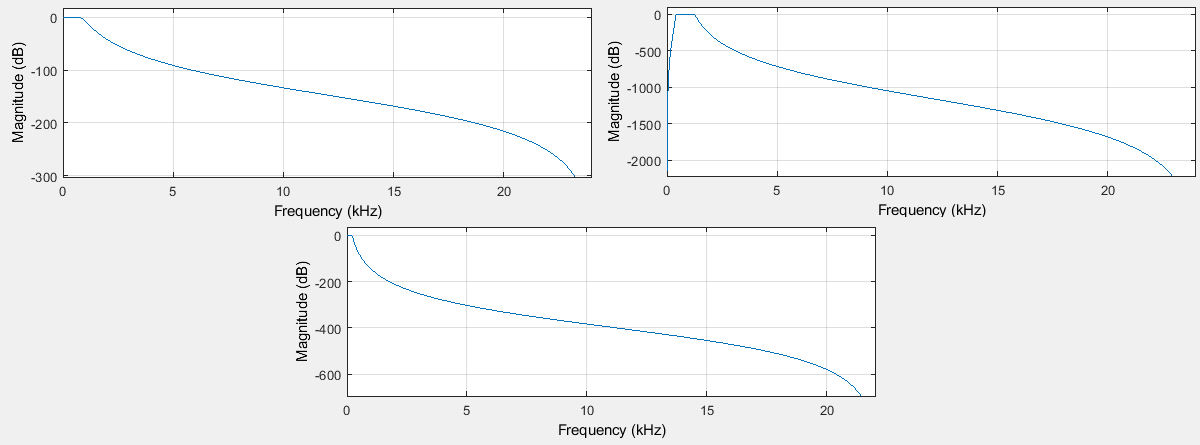
\includegraphics[width=\linewidth]{filters}    	
	\caption{Left-to-right: The filters used for Sweet Child O Mine guitar, Comfortably Numb bass, Comfortably Numb solo}
	\label{fig:filters}
\end{figure}

\subsubsection{Spectrogram}

The output of the Gabor Transform is well-displayed via spectrogram. This has time on the horizontal axis, frequency on the vertical axis, and at all points between these axes, the signal power at that frequency and that time is plotted in color.

\subsubsection{Scientific frequency vs musical pitch}
A frequency can be converted into the note it most closely matches. This note can be displayed in standard scientific notation (e.g. \texttt{C4}), or it can be displayed in a manner corresponding to how the MIDI (Musical Instrument Digital Interface) protocol stores notes as 7-bit integers. The note \texttt{C4} is stored as $60$ in base-10, and a change in semitones is stored as a corresponding change (e.g. \texttt{C5} is $+12$ semitones higher, so it is stored as $72$). This is useful for easily plotting a transcription without regards for musical notation.


% Algorithm Implementation and Development
\section{Algorithm Implementation and Development}


\subsection{Filtering}

For the guitar in the Guns N Roses sample, I apply a weak low-pass filter to curb the overtones before transcribing.

For the bass in the Pink Floyd sample, I apply a strong low-pass filter to isolate the bass in the mix, particularly to avoid the rhythm guitar.

For the lead guitar in the Pink Floyd sample, I apply a strong band-pass filter to isolate the solo, particularly to avoid the overtones of the bass and rhythm guitar.


\subsection{Transcribing}
The process of transcription begins by computing the spectrogram with Algorithm~\ref{alg:gabors}. Then, the frequency bin with maximum power in each column is mapped to the corresponding note. Sequential instants with the same note are regarded as a single extended note (e.g. \texttt{[F\#5, F\#5, G5, D\#5, D\#5]} $\longrightarrow$ \texttt{[F\#5, G5, D\#5]})

Filters are designed, generated, and applied via MATLAB's Signal Processing Toolbox.



The parameter $T$ is calibrated with regards to performance and memory consumption. The parameter $\alpha$ is calibrated with regards to subsection~\ref{sct:heisenberg}.

See Appendix A for more subroutines written to clean the resulting output into a human-presentable form.


\begin{algorithm}[!t]
\begin{algorithmic}
	\STATE{Initialize Gaussian function $g(t, \tau)=e^{a(t-\tau)^2}$}
	\STATE{Compute $y_t = x_tg(t,\tau)$}
	\STATE{Compute and return the DFT of $y_t$}
\end{algorithmic}
\caption{Gabor Transform($x_t,\alpha,\tau$)}
\label{alg:gabor}
\end{algorithm}

\begin{algorithm}[!t]
	\begin{algorithmic}
		\STATE{Initialize an empty solution matrix with dimensions of length($x_t$) and length($T$)}
		\FORALL{$\tau \in T$}
		\STATE{Store Gabor Transform($x_n,\alpha,\tau$) (Algorithm~\ref{alg:gabor})} as a column in the solution matrix 
		\ENDFOR{}
		\STATE{Return the solution matrix.}
	\end{algorithmic}
	\caption{Spectrogram($x_t, \alpha, T$)}
	\label{alg:gabors}
\end{algorithm}

% Computational Results
\section{Computational Results}

\begin{figure}[!h]
	\centering
	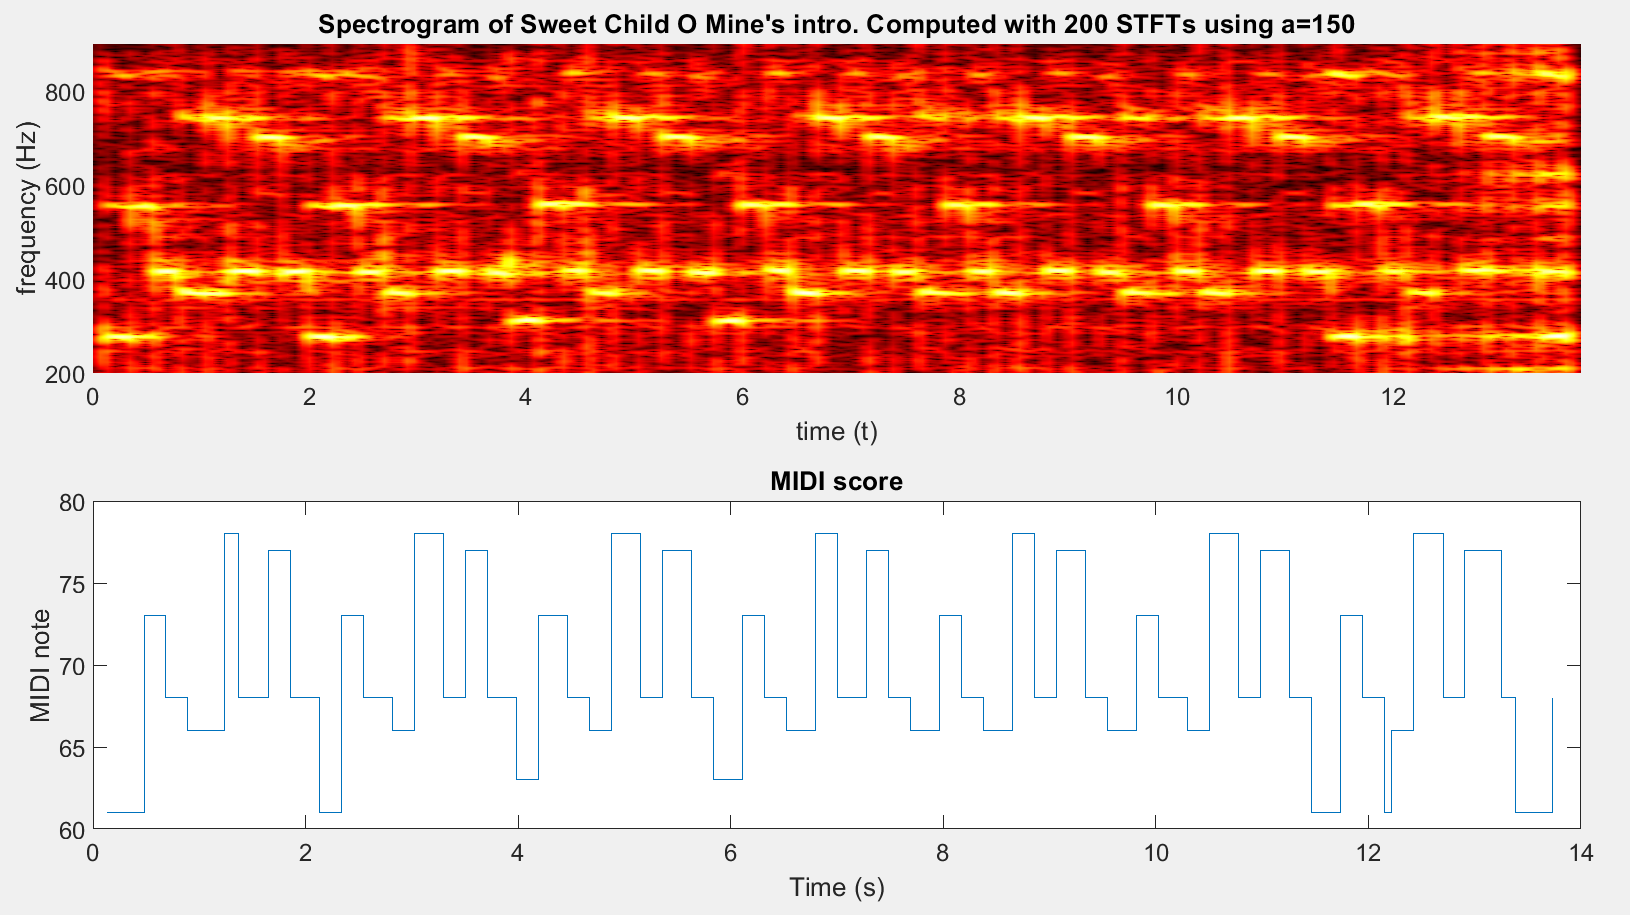
\includegraphics[width=\linewidth]{score_1}    	
	\caption{Analysis of Guns N Roses riff}
	\label{fig:spect2}
\end{figure}


\begin{figure}[!h]
	\centering
	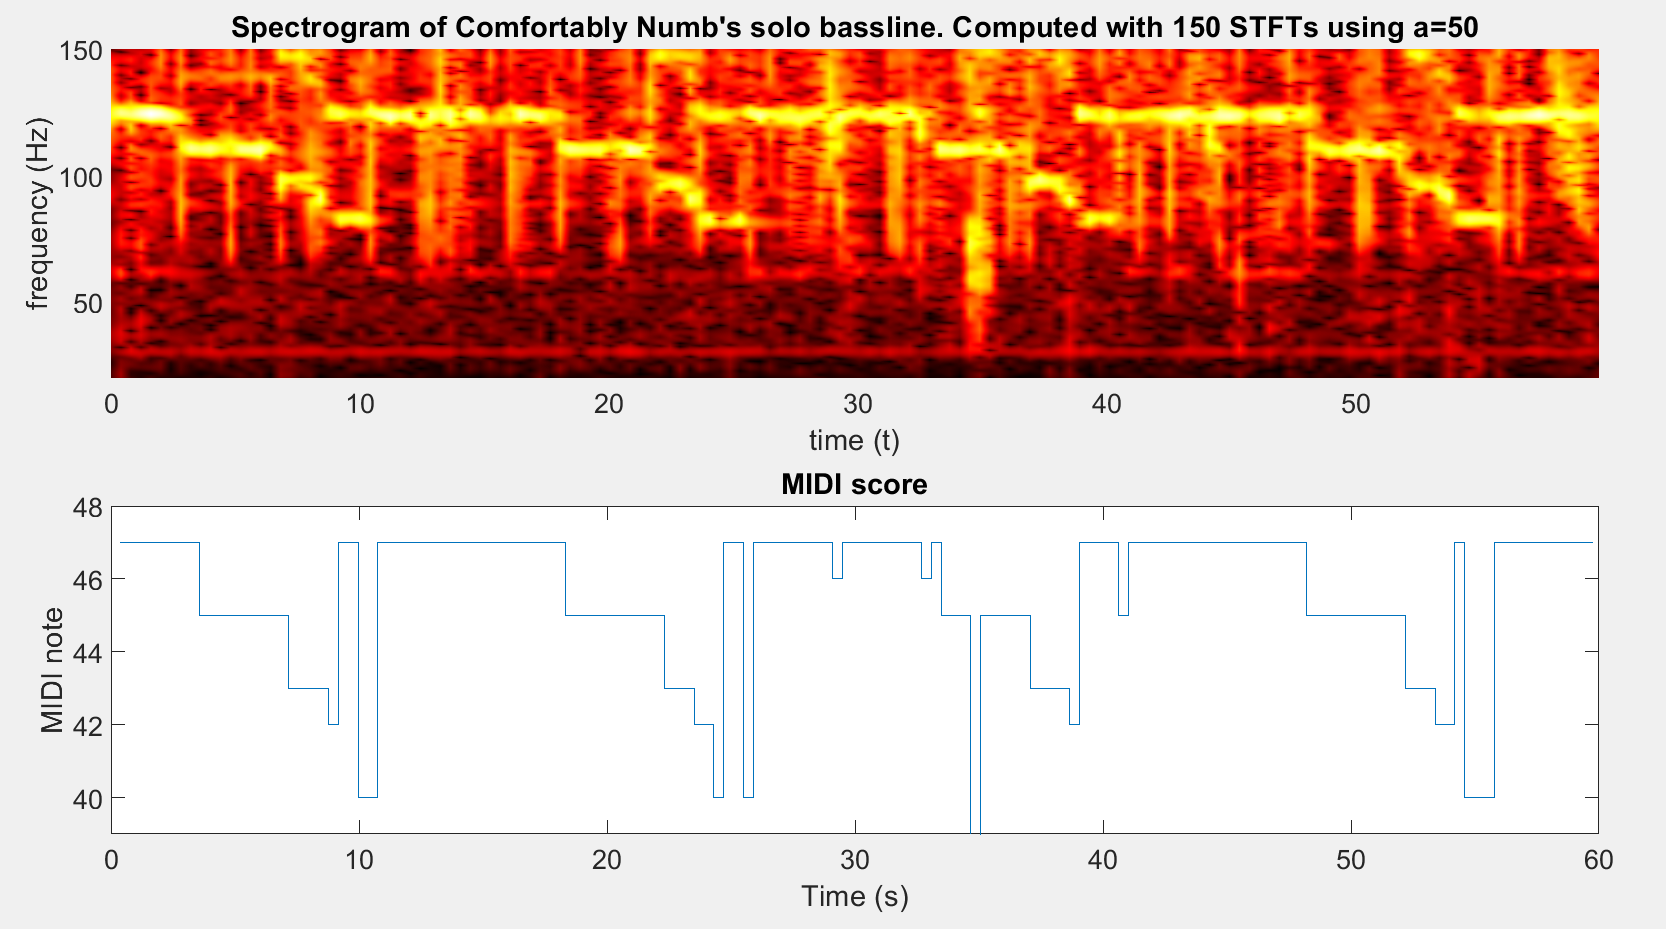
\includegraphics[width=\linewidth]{score_2}    	
	\caption{Analysis of low-pass filtered Pink Floyd bassline during solo}
	\label{fig:spect2}
\end{figure}

\begin{figure}[!t]
	\centering
	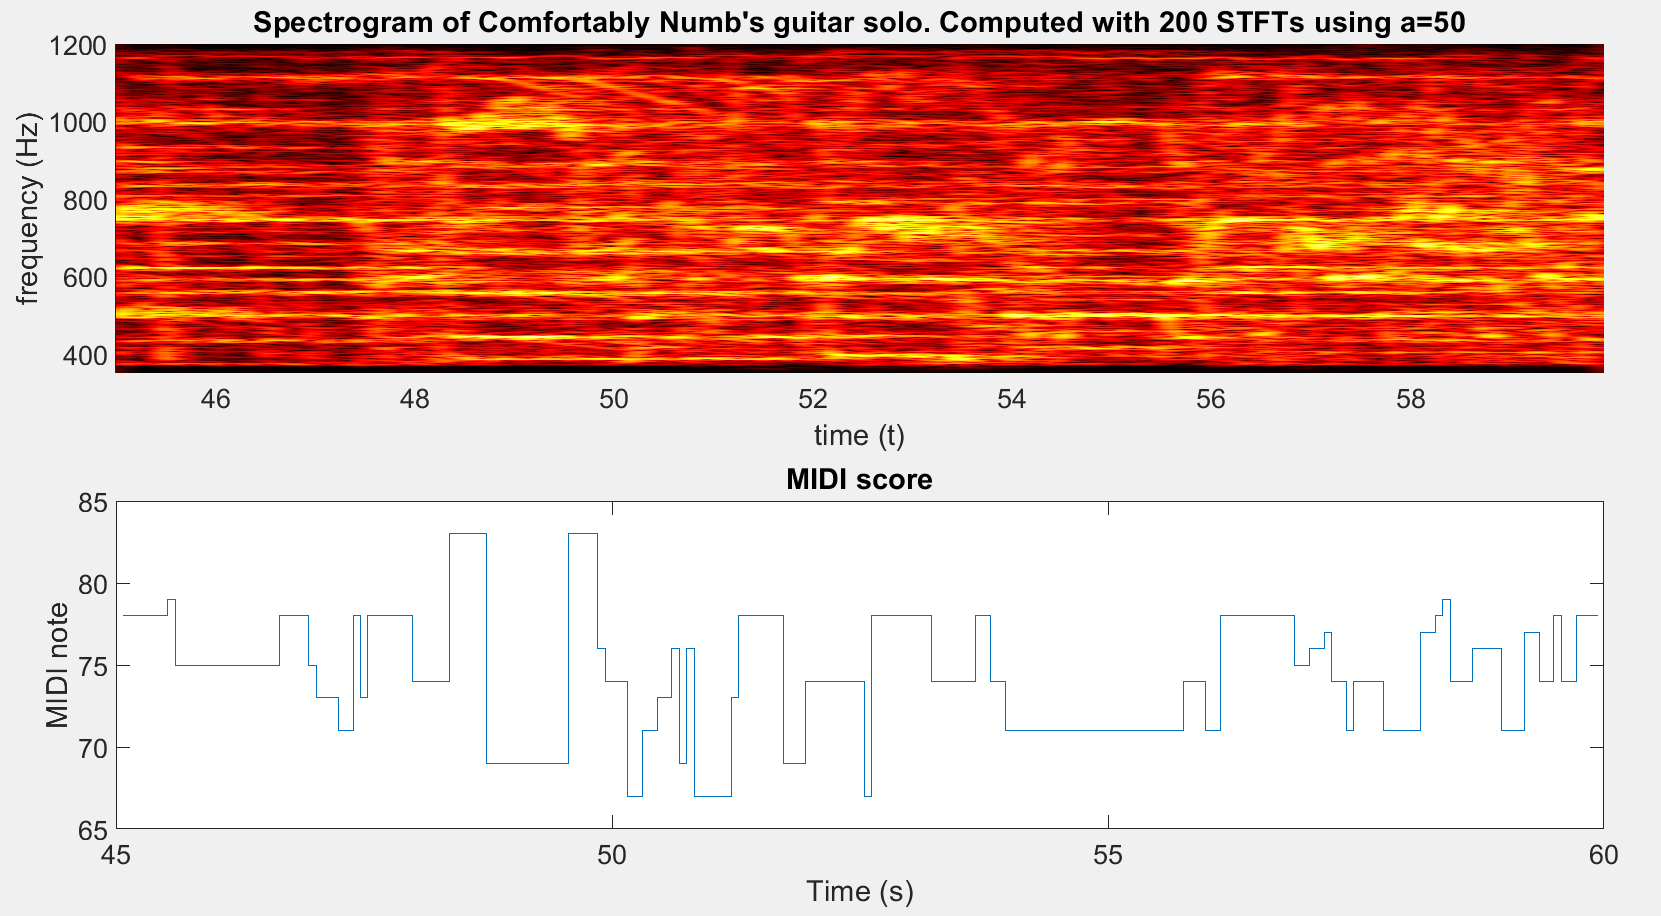
\includegraphics[width=\linewidth]{score_3}    	
	\caption{Analysis of last 15 seconds of band-pass filtered Pink Floyd guitar solo}
	\label{fig:spect2}
\end{figure}

\begin{figure}[]
	\centering
	\begin{subfigure}{.35\textwidth}
		\centering
		\begin{lstlisting}[basicstyle=\small]
B2,A2,G2,F#2,B2,E2,
B2,A2,G2,F#2,E2,B2,E2,
B2,A#2,B2,A#2,
B2,A2,D2,A2,G2,F#2,
B2,A2,B2,A2,G2,F#2,
B2,E2,B2
		\end{lstlisting}
		\caption{Sweet Child O Mine riff}
	\end{subfigure}%
	\begin{subfigure}{.35\textwidth}
		\centering
			\begin{lstlisting}[basicstyle=\small]
C#4,C#5,G#4,F#4,F#5,G#4,F5,G#4,
C#4,C#5,G#4,F#4,F#5,G#4,F5,G#4,
D#4,C#5,G#4,F#4,F#5,G#4,F5,G#4,
D#4,C#5,G#4,F#4,F#5,G#4,F5,G#4,
F#4,C#5,G#4,F#4,F#5,G#4,F5,G#4,
F#4,C#5,G#4,F#4,F#5,G#4,F5,G#4,
C#4,C#5,G#4,C#4,F#4,F#5,G#4,F5,
G#4,C#4
			\end{lstlisting}
		\caption{Comfortably Numb bass}
	\end{subfigure}
	\begin{subfigure}{.35\textwidth}
		\centering
		\begin{lstlisting}[basicstyle=\small]
F#5,G5,D#5,F#5,D#5,C#5,B4,F#5,
C#5,F#5,D5,B5,A4,B5,E5,D5,
G4,B4,C#5,E5,A4,E5,G4,C#5,
F#5,A4,D5,G4,F#5,D5,F#5,D5,
B4,D5,B4,F#5,D#5,E5,F5,D5,
B4,D5,B4,F5,F#5,G5,D5,E5,
B4,F5,D5,F#5,D5,F#5
		\end{lstlisting}
	\caption{Comfortably Numb solo excerpt}
		\end{subfigure}
	\caption{Song transcriptions}
	\label{fig:transcriptions}
\end{figure}
\newpage
% Summary and Conclusions
\;
\;
\;
\;

\;
\;
\section{Summary and Conclusions}
The method of filtering and applying the Gabor transform can be useful for music transcription of isolated instruments. It works very well for the Guns N Roses riff, with perfect transcription up until the last two seconds where other instruments vamp in. 

This method also works fairly well for the filtered Pink Floyd bassline, though this has some artifacts which can be seen as large oscillating jumps of semitones. This could possibly be improved with numerical optimization of the Gabor parameters to minimize "jumpiness" in the score.

This method unfortunately does not work well with the Comfortably Numb solo. One reason could be because some of the notes are played very quickly, and the frequency-time analysis just can't get enough time resolution without sacrificing excessive frequency resolution. However, the transcription also does not seem to capture the long notes well despite my best efforts to adjust the filter cutoffs. 

I conclude that the method of simply filtering and computing Gabor transform is too simplistic for dealing with a dense mix, though it does succeed in dealing with isolated instruments with dense harmonic spectrums as demonstrated with Guns N Roses.


One application could include a Digital Audio Workstation VST plugin which reads in isolated audio of an instrument playing, filters it, and transcribes the dominant frequencies. Because I am able to compute a Gabor transform of 60 seconds of music in significantly less than 60 seconds, this can be implemented in almost real-time, though in order to compute a Gabor transform, a window might be needed which, unlike the Gaussian window, reaches zero; a Hamming window would do. In that case, near real-time music transcription could be implemented with a delay equal to the width of the window.  

% References
\printbibliography

% Appendices
\begin{appendices}

% MATLAB Functions
\section{MATLAB Functions}

\begin{itemize}
    \item \texttt{note = freq2note(freq)} inputs a vector of frequencies. It computes the frequencies' relative pitch via modular arithmetic and relative octave via division, all relative to the base note \texttt{C0}, and outputs as a vector of strings.
    
    \item \texttt{note = freq2midi(freq)} inputs a vector of frequencies. It computes the number of semitones each frequency is above \texttt{C0}, and uses that to return the MIDI pitch values as a vector of integers.
    
    \item \texttt{notes = removeDuplicate(notes\_raw)} inputs a vector of notes (as strings). If two or more adjacent notes have the same value, it quashes them into one note.
    
    \item The following methods respectively apply the filters designed for Sweet Child O Mine guitar, Comfortably Numb bass, and Comfortably Numb solo
    
    \begin{itemize}
       	\item \texttt{y\_f = gnrlowpass48(y)}
    	\item \texttt{y\_f = bassFilter(y)}
    	\item \texttt{y\_f = soloFilter(y)} 
    \end{itemize}
\end{itemize}

% MATLAB Codes
\section{MATLAB Code}

\subsection{main.m}

\inputminted{matlab}{main.m}
\subsection{freq2midi.m}
\inputminted{matlab}{freq2midi.m}
\subsection{freq2note.m}
\inputminted{matlab}{freq2note.m}
\subsection{gnrlowpass48.m}
\inputminted{matlab}{gnrlowpass48.m}
\subsection{lowpassbass.m}
\inputminted{matlab}{lowpassbass.m}
\subsection{removeDuplicate.m}
\inputminted{matlab}{removeDuplicate.m}

\end{appendices}

\end{document}